\documentclass[11pt]{article}

\usepackage[margin=1in]{geometry}
\usepackage{amsmath,amssymb}
\usepackage{graphicx}
\usepackage[colorlinks=true,linkcolor=blue!50!black,urlcolor=blue!50!black]{hyperref}
\usepackage{booktabs}
\usepackage{tabularx}
\usepackage{xcolor}
\usepackage{array}
\usepackage{enumitem}
\usepackage{float}
\usepackage{caption}
\setlist{itemsep=2pt,topsep=4pt}
\newcolumntype{Y}{>{\raggedright\arraybackslash}X}
\newcommand{\figw}{\textwidth}
\newenvironment{keybox}{\par\smallskip\noindent\begin{minipage}{\textwidth}\color{black}\itshape}{\end{minipage}\par\smallskip}

\title{Project Summary: Recursive Computation Under Action Delay\\[2pt]
\large Phases 1--2 and the Phase 3 Plan}
\author{\texttt{trm-delay-robust-scaling}}
\date{17 September 2026}

\begin{document}
\maketitle

\noindent\small Sources: \texttt{papers/phase1/report.md}, \texttt{papers/phase2/report.md}, the combined report \texttt{papers/report.md} (including its post-hoc mechanistic analysis), and the Phase 3 plan \texttt{papers/phase3/plan.md}. Section~\ref{sec:review} is a review of that plan against the codebase. Figures 11--12 are new (\texttt{experiments/make\_figures\_summary.py}).\normalsize

\section*{The short version}

\begin{itemize}
  \item \textbf{The question.} Tiny Recursive Models (TRM) beat much larger networks on puzzle benchmarks by running one small shared cell over and over, instead of adding parameters. \emph{Does that trade (iterations instead of parameters) still pay off when the network is the actor/critic trunk of a model-free RL agent controlling a plant with delayed actions?}
  \item \textbf{Phase 1} (48 runs: Pendulum-v1 and MountainCarContinuous-v0, 4 trunks, 0- and 1-step delay) tested whether TRM's disadvantage shrinks as horizon and reward sparsity grow. \textbf{TRM was significantly \emph{worse} than a $5.8\times$ smaller MLP on Pendulum (6/6 seed-pairs, $p=0.016$).} It tied on MountainCar. The pre-registered threshold prediction was falsified.
  \item \textbf{Phase 2} (54 runs: BipedalWalker-v3, 6 trunks including two more TRM variants, plus an augmentation ablation) tested a second complexity axis: dimensionality and dynamics coupling. \textbf{No comparison reached significance in any direction.} TRM cost 5--$8\times$ the MLP's wall-clock.
  \item \textbf{Post-hoc analysis} of all 102 runs changed what the headline means. (i) Two of the three environments are \textbf{floor effects}: no architecture learned them. (ii) The recursive trunks \textbf{fit the value function worse} (7/7 cells, $p=0.008$), but a similarly-sized Transformer does too and a small LSTM does not. The deficit \textbf{tracks parameter count, not recursion}. (iii) The TRM port \textbf{resets its latent every forward call}, the weaker of two variants that independent work compared directly.
  \item \textbf{Phase 3} stops adding environments. It (a) removes the three confounds, (b) tests recursion where it \emph{could} help, and (c) adds a control-engineering scorecard: command smoothness, robustness margins, and inference latency. Stages are gated; only a cheap Stage~0 is committed.
  \item \textbf{Review verdict (\S\ref{sec:review}).} The plan's diagnosis and gated structure are strong. But \textbf{its decisive condition, stochastic delay with augmentation, turns out to contain no hidden state in this codebase.} I verified this against \texttt{DelayedEnv}: the applied action was always visible to the agent in 19{,}600 of 19{,}600 steps, and the delay is drawn fresh and independently each step. As written, Stage~0's headroom gate and Stage~2's interaction test would return a null \emph{whether or not} the hypothesis is true. \S\ref{sec:amend} gives a concrete redesign.
\end{itemize}

\section{Background: why this question, and why delay}

\textbf{TRM's claim.} A roughly 7M-parameter, two-layer, weight-tied cell reaches 45\% on ARC-AGI-1 and 87\% on Sudoku-Extreme, beating far larger models (Jolicoeur-Martineau, 2025). The implied claim is about a \emph{computational mechanism}: iteration depth with tied weights can substitute for parameter count. If that is true, it should matter in places other than puzzles, such as embedded and robotic control, where parameters, memory and latency are all scarce.

\textbf{Why action delay is a fair test.} Under a $d$-step action delay, what happens at time $t$ was caused by the action chosen $d$ steps earlier, so the raw observation is no longer Markov. The classical fix is \textbf{observation augmentation}: append the queue of actions that have been committed but not yet applied. This restores a sufficient statistic (Katsikopoulos \& Engelbrecht, 2003). That theorem only says such a statistic \emph{exists}, though, not that a small network can \emph{fit} the resulting value function efficiently. The project's founding bet was that iterative latent refinement (something like a learned state estimator) would be a better inductive bias for that fitting problem than a single feed-forward pass.

\textbf{What gets compared.} Every trunk is a drop-in feature extractor for both actor and critic under DDPG, so the trunk is the only thing that changes. Reward, wall-clock time and parameter count are reported as \textbf{co-equal} metrics.

\begin{table}[H]
\centering\small
\begin{tabularx}{\textwidth}{lrY}
\toprule
Trunk & Params (actor+critic, Pendulum) & Mechanism \\
\midrule
DNN [256, 256] & 134,914 & memoryless MLP baseline \\
LSTM & 166,562 & recurrence within a call, stateless across steps (mechanistic control) \\
TRM (base) & 787,842 & weight-tied recursion, \texttt{H\_cycles}=3 $\times$ \texttt{L\_cycles}=6, two latents \\
TRM-hier6 & 787,842 & six parallel low-level latent slots (Phase 2) \\
TRM-singlez & 787,842 & a single latent, no $z_H$/$z_L$ split (Phase 2) \\
Transformer & 797,058 & per-feature self-attention \\
\bottomrule
\end{tabularx}
\end{table}

\section{Phase 1 --- Does TRM's disadvantage shrink as the horizon grows?}

\subsection{What was done}
An informal pilot on Pendulum-v1 suggested TRM, a Transformer and an MLP reached ``comparable reward'' under 1-step delay, with TRM costing about $18\times$ the MLP's training time. Phase 1 did not conclude that recursion is useless. It asked whether \textbf{Pendulum is simply too easy to reward extra computation}, and turned that into a falsifiable hypothesis:

\begin{quote}
\textbf{H1:} TRM's advantage over the MLP and Transformer is non-decreasing in task complexity. \textbf{Pre-registered threshold:} it becomes measurable once the horizon is roughly $5\times$ Pendulum's \emph{and} reward is sparse, which is what MountainCarContinuous-v0 provides (999 steps, one sparse terminal reward).
\end{quote}

\begin{itemize}
  \item \textbf{Design:} 4 trunks $\times$ 2 environments $\times$ 2 delay conditions (0-step; 1-step + augmentation) $\times$ 3 seeds $=$ \textbf{48 runs}, 200 episodes each, CPU-only on Katana.
  \item \textbf{Statistic:} a pooled one-sided sign test on per-seed reward differences, $n=6$ per comparison, so 5/6 or 6/6 gives $p\le0.031$. This replaced an earlier regression design that review showed could never get below $p=0.125$ at $n=3$.
\end{itemize}

\subsection{Why it mattered}
It turned an anecdote (``TRM ties but is slower'') into a controlled, pre-registered measurement. It also tested the most natural rescue of the pilot (``harder tasks will need the extra computation'') \emph{before} more compute went into it.

\subsection{Findings}
\begin{table}[H]
\centering\small
\begin{tabular}{llrr}
\toprule
Comparison & Environment & TRM wins / 6 & one-sided $p$ \\
\midrule
TRM $-$ DNN & Pendulum-v1 & \textbf{0/6} & \textbf{0.016} (significant \emph{deficit}) \\
TRM $-$ DNN & MountainCarContinuous-v0 & 3/6 & 0.656 \\
TRM $-$ Transformer & Pendulum-v1 & 3/6 & 0.656 \\
TRM $-$ Transformer & MountainCarContinuous-v0 & 4/6 & 0.344 \\
\bottomrule
\end{tabular}
\end{table}

\begin{enumerate}
  \item \textbf{The pilot was wrong about parity.} With the full replication, the MLP beat TRM in every seed-pair on Pendulum, by 37 reward units under fixed delay ($-194.0$ vs $-231.1$). That is about 3\% of the gap between an untrained policy ($\approx-1460$) and the best run: consistent, but small.
  \item \textbf{The gap closed on MountainCar and moved in the predicted direction} (median TRM$-$DNN from $-28.3$ to $+0.4$; TRM$-$Transformer from $+3.2$ to $+23.3$), but never reached significance. The threshold prediction was \textbf{falsified}; the general hypothesis was left open.
  \item \textbf{The cost grew with complexity:} TRM went from ${\sim}7\times$ to ${\sim}13$--$14\times$ the MLP's wall-clock.
  \item The LSTM never learned Pendulum ($\approx-1460$) but learned the other tasks normally. This was flagged as a tuning artefact rather than evidence about recurrence (Ni et al., 2022).
\end{enumerate}

\begin{figure}[H]\centering
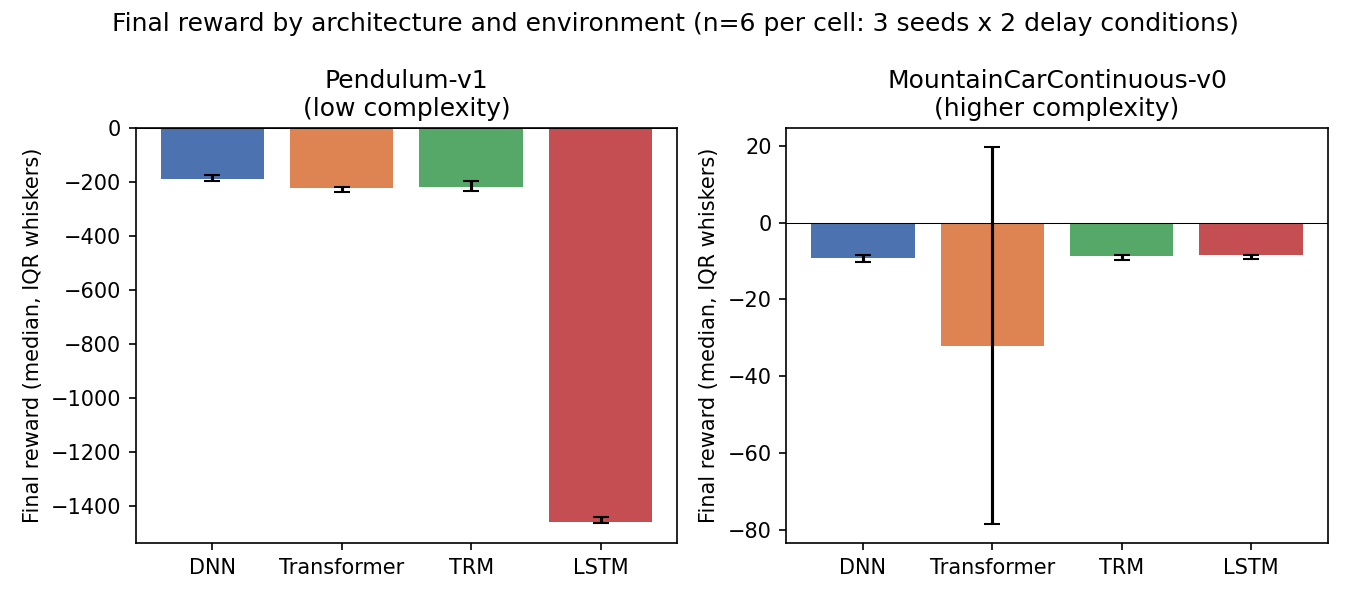
\includegraphics[width=0.49\textwidth]{figures/fig1_reward_by_arch_env.png}\hfill
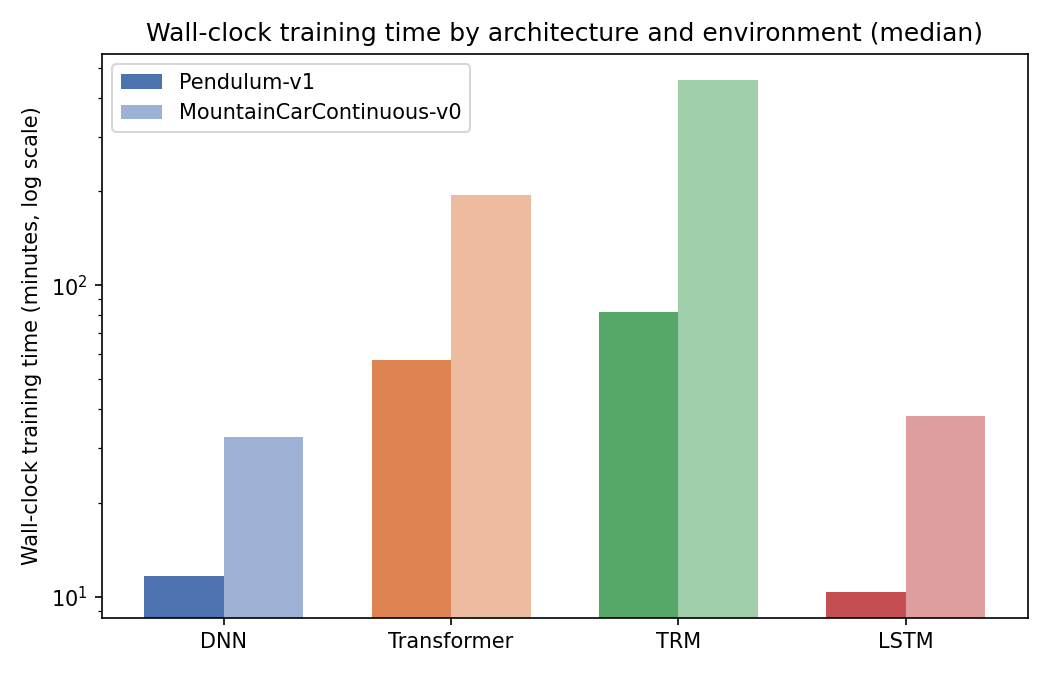
\includegraphics[width=0.49\textwidth]{figures/fig2_wallclock_by_arch_env.png}
\caption{Phase 1: final reward (left) and wall-clock training time (right) by trunk and environment.}
\end{figure}

\begin{figure}[H]\centering
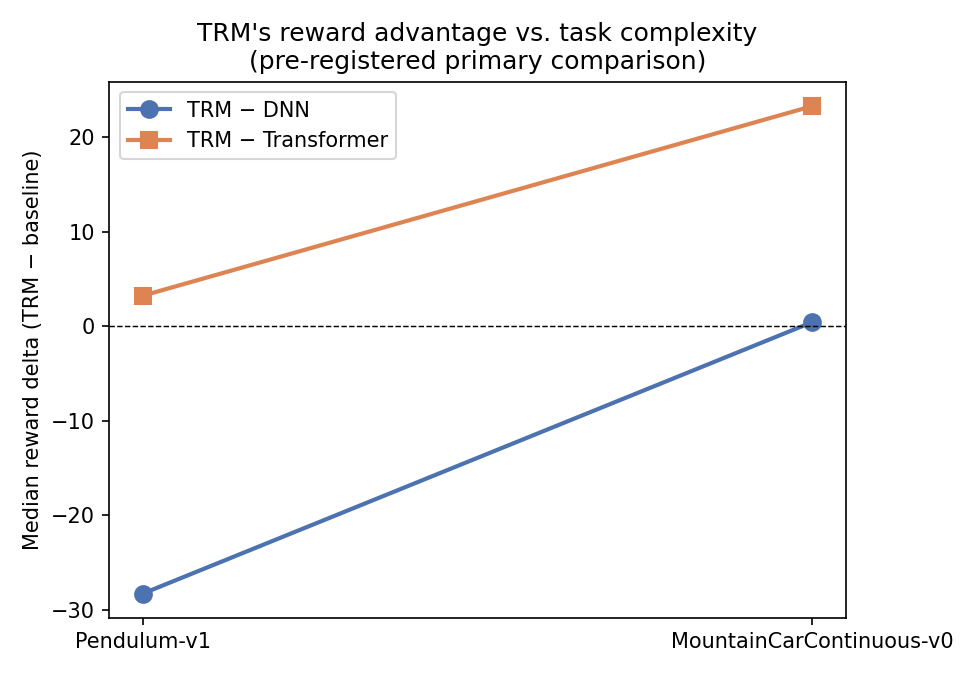
\includegraphics[width=0.55\textwidth]{figures/fig3_trm_advantage_trend.png}
\caption{Phase 1: TRM's median reward advantage vs task complexity. It moves in the hypothesised direction but is never significant.}
\end{figure}

\section{Phase 2 --- A second complexity axis: dimensionality and coupling}

\subsection{What was done}
Phase 1 covered one complexity axis (horizon and sparsity). Its pre-committed next step was a \emph{different} axis, so that the two phases together could not be read as restating one test.
\begin{itemize}
  \item \textbf{Environment:} BipedalWalker-v3 (24-D observation, 4-D action, coupled underactuated dynamics).
  \item \textbf{Trunks:} the four from Phase 1 plus \textbf{TRM-hier6} and \textbf{TRM-singlez}, to test whether the result depended on TRM's \emph{particular} recursive structure.
  \item \textbf{Conditions:} no delay; 1-step delay + augmentation; \textbf{1-step delay without augmentation}.
  \item \textbf{Scale:} $6\times3\times3$ seeds $=$ \textbf{54 runs}, one V100 each. A filename collision silently overwrote three DNN cells. QA caught it before analysis and the six jobs were re-run.
\end{itemize}

\subsection{Why it mattered}
It was the pre-registered falsification rung: if neither axis showed a TRM advantage, the general complexity-scaling hypothesis would count as disconfirmed. It also added the first \textbf{structure ablation} and the first \textbf{augmentation ablation}.

\subsection{Findings}
\begin{table}[H]
\centering\small
\begin{tabular}{lrlr}
\toprule
Comparison (fixed + aug, $n=3$) & TRM wins & per-seed $\Delta$ & one-sided $p$ \\
\midrule
TRM $-$ DNN & 2/3 & $+6.3,\ -10.8,\ +8.7$ & 0.5 \\
TRM $-$ Transformer & 0/3 & $-14.4,\ -0.9,\ -14.7$ & 0.125 \\
TRM $-$ LSTM & 1/3 & $-1.1,\ -3.5,\ +3.9$ & 0.5 \\
\bottomrule
\end{tabular}
\end{table}

\begin{enumerate}
  \item \textbf{Nothing was significant in any direction.} Taken with Phase 1, the project had covered two complexity axes on three environments \textbf{without a single significant TRM advantage}.
  \item \textbf{The recursive structure made no detectable difference.} Base vs hier6 vs singlez deltas changed sign seed to seed; both variants cost \emph{more} than the base TRM.
  \item \textbf{Augmentation had no clear effect for any trunk.} Two candidate signals hit the $n=3$ ceiling ($p=0.125$): TRM-hier6 helped by augmentation in 3/3 seeds, LSTM hurt in 3/3. They were flagged for a powered follow-up, not reported as findings.
  \item \textbf{The cost stayed high:} TRM $5.2\times$, hier6 $6.9\times$, singlez $8.0\times$ the MLP's wall-clock.
\end{enumerate}

\begin{figure}[H]\centering
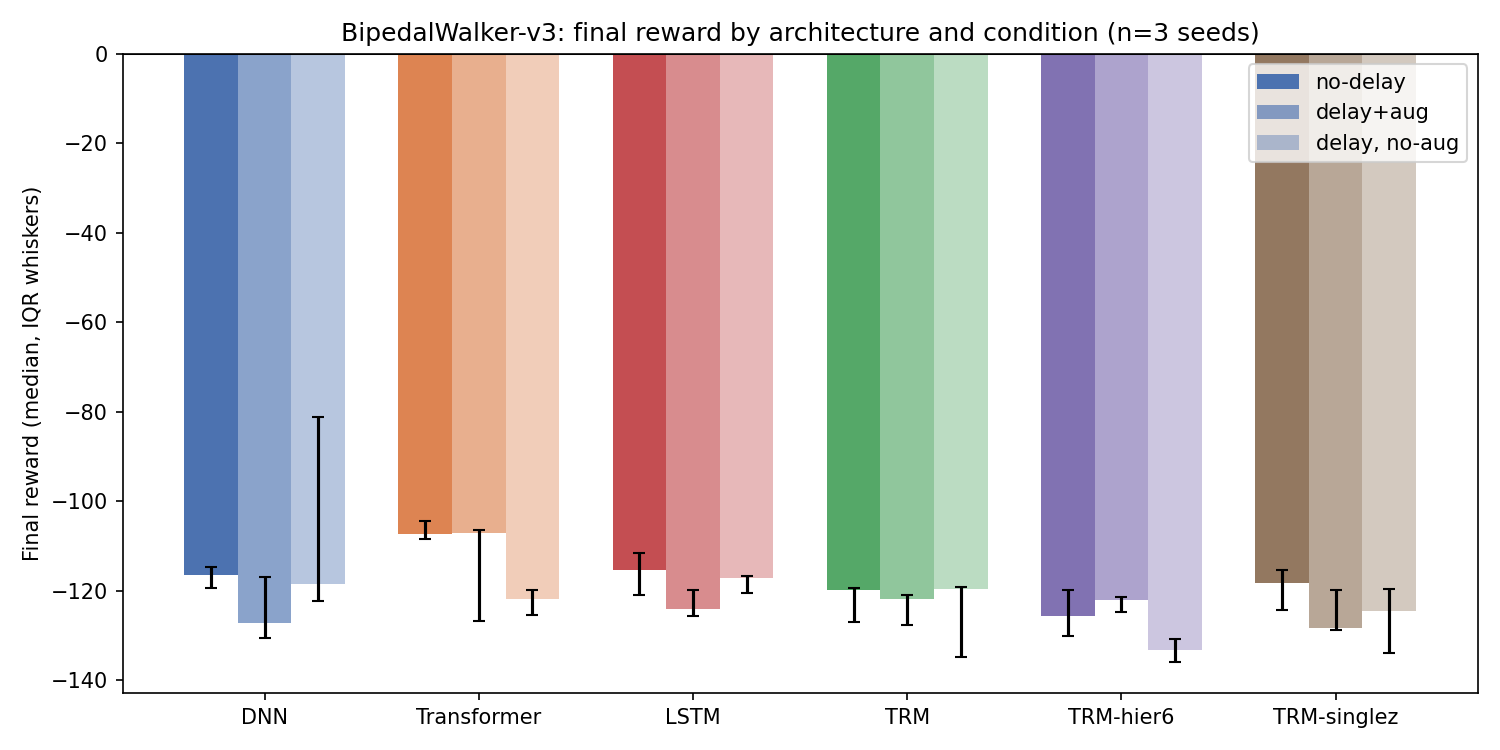
\includegraphics[width=0.49\textwidth]{figures/fig4_reward_by_arch_cond.png}\hfill
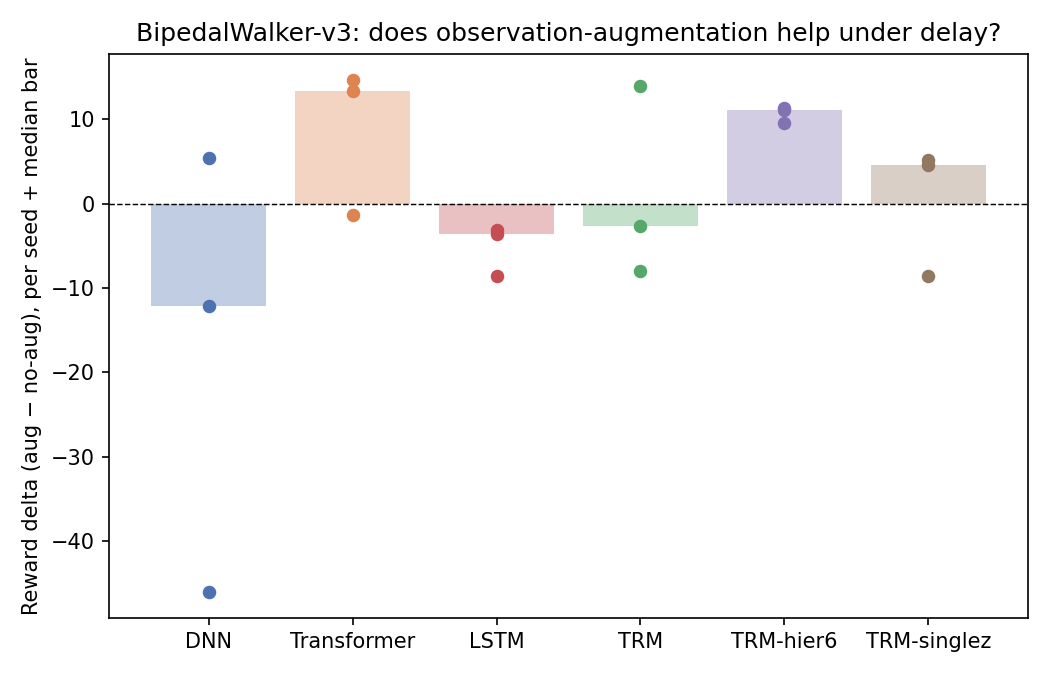
\includegraphics[width=0.49\textwidth]{figures/fig7_augmentation_ablation.png}
\caption{Phase 2 (BipedalWalker-v3): final reward by trunk and condition (left); augmentation ablation, per-seed deltas (right).}
\end{figure}

\begin{figure}[H]\centering
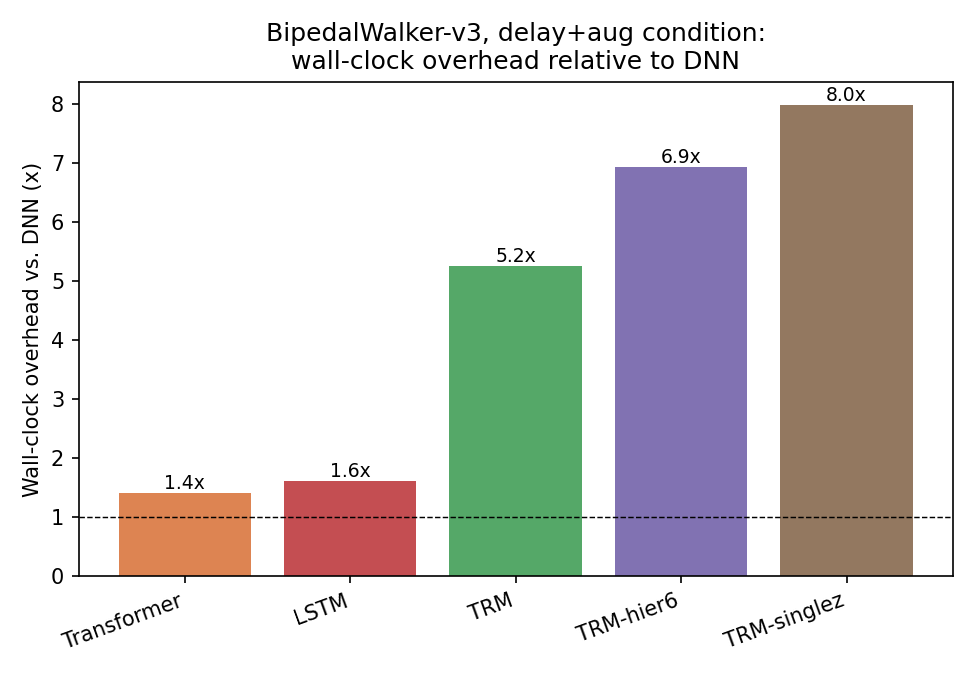
\includegraphics[width=0.6\textwidth]{figures/fig6_trm_overhead.png}
\caption{TRM-family wall-clock overhead relative to the MLP.}
\end{figure}

\section{Post-hoc analysis --- what Phases 1--2 actually established}

After Phase 2, the combined report re-analysed all 102 runs using the per-episode telemetry (returns, actor loss, critic loss) every run had already logged. No new compute was used. This step is where the project changed its understanding of its own results, and it is the reason Phase 3 looks the way it does.

\subsection{Two of the three environments are floor effects}
\begin{table}[H]
\centering\small
\begin{tabularx}{\textwidth}{lrrrY}
\toprule
Environment & Solved & Best final & Median final & Verdict \\
\midrule
Pendulum-v1 & $\approx-150$ & $-169.9$ & $-219.9$ & \textbf{learned} \\
MountainCarContinuous-v0 & $+90$ & $+45.6$ & $-8.9$ & exploration-limited (known DDPG + OU failure; Matheron et al., 2019) \\
BipedalWalker-v3 & $+300$ & $-81.1$ & $-120.7$ & \textbf{floor}: no run learned to walk \\
\bottomrule
\end{tabularx}
\end{table}
\textbf{Why this matters:} ``the gap closes as tasks get harder'' is exactly what you see when \emph{no} architecture learns and every result collapses onto the same floor. The complexity-scaling question was \textbf{never put at risk}. It is untested, not disconfirmed. Pendulum is the only valid comparison in the study.

\subsection{Recursive trunks fit the value function worse, and so does the Transformer}
At the same episode budget, TRM's critic loss was higher than the MLP's in \textbf{7/7 cells early in training (median $2.72\times$, $p=0.008$)}; across the three TRM variants, 13/13. Learning speed and stability did \emph{not} differ (episodes to 90\%: 117 vs 115 on Pendulum; seed spread not inflated). TRM follows the same trajectory to a slightly lower plateau.

\begin{figure}[H]\centering
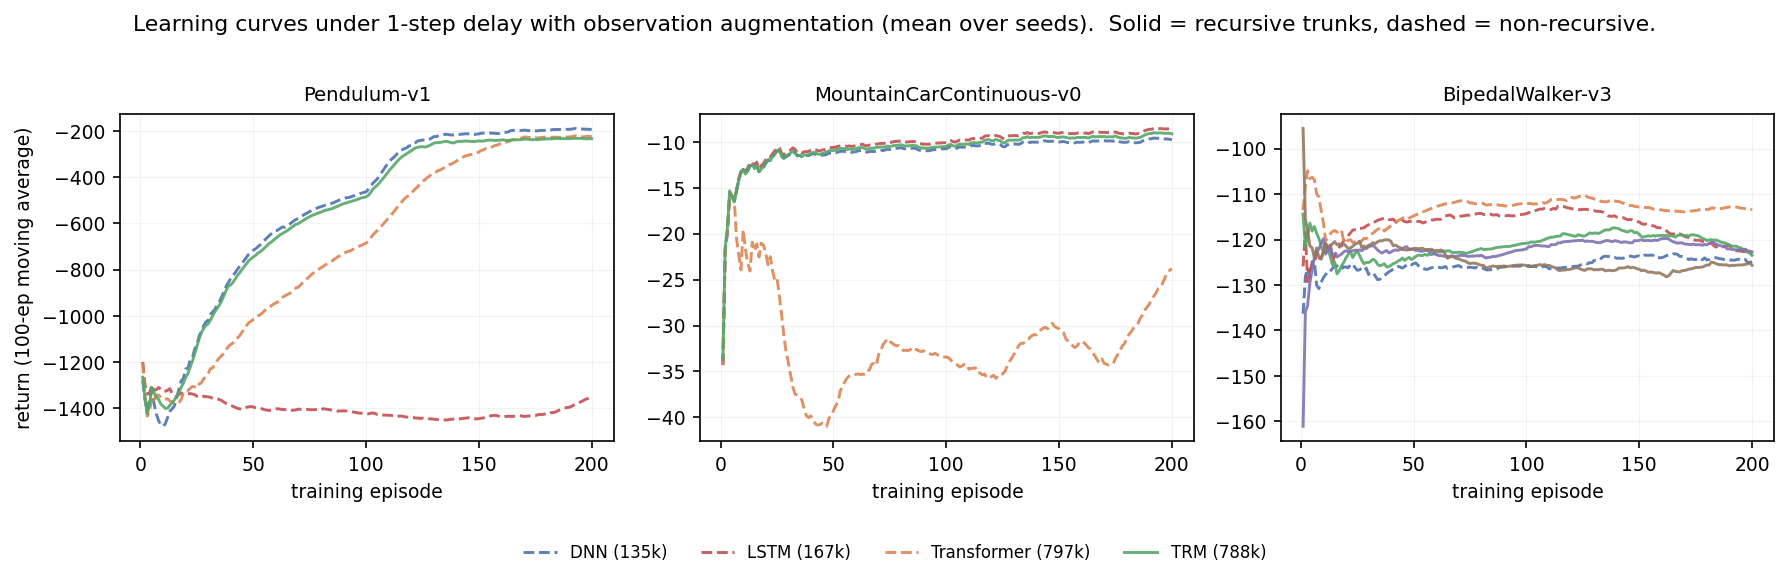
\includegraphics[width=\figw]{figures/fig8_learning_curves.png}
\caption{Learning curves under 1-step delay with augmentation.}
\end{figure}

\textbf{The same deficit appears in the 797k Transformer (6/7 early, 7/7 late) and not in the 167k LSTM (3/7, $0.95\times$).} Sorted by parameter count, the value-fit deficit follows \emph{size}, not recursion. This matches a known deep-RL result: naively scaling capacity does not help and can hurt (Ota et al., 2021; Klein et al., 2024).

\begin{figure}[H]\centering
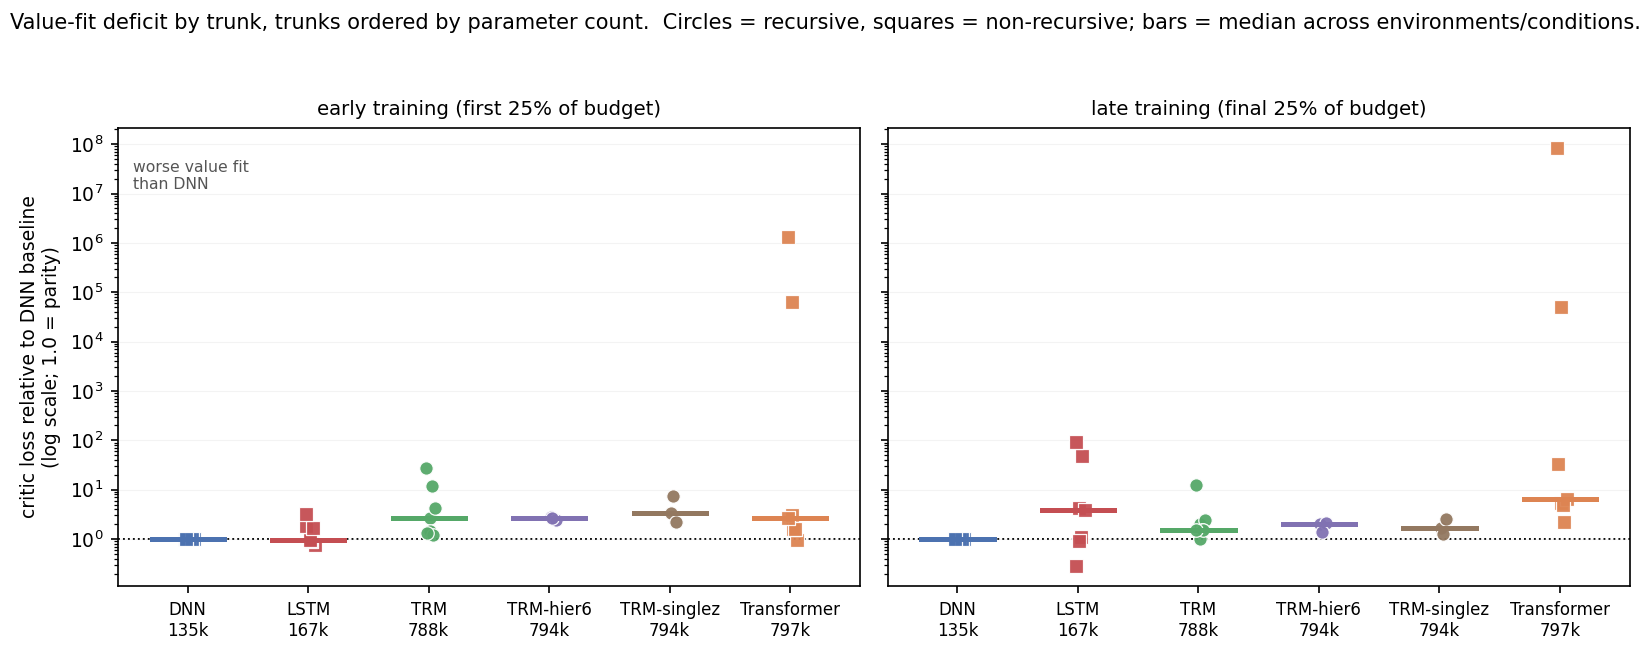
\includegraphics[width=\figw]{figures/fig10_capacity_vs_valuefit.png}
\caption{Value-fit deficit by trunk, ordered by parameter count.}
\end{figure}

\subsection{The three confounds}
\begin{itemize}
  \item \textbf{C-1, capacity.} Every recursive trunk has ${\approx}788$k parameters; the MLP has 135k. Nothing in the design separates the two, and the evidence currently favours capacity as the explanation.
  \item \textbf{C-2, latent reset.} \texttt{TRMTrunk.forward} re-initialises $z_H$/$z_L$ from fixed buffers on every call, so nothing carries across control steps. HRM-Agent (Dang \& Rawlinson, 2025), which trained a recursive reasoning model with RL alone \emph{and succeeded}, found that carrying the latent (``Carry-Z'') beats resetting it. \textbf{A trunk with no cross-step state cannot do state estimation.}
  \item \textbf{C-3, nothing to infer.} Under fixed 1-step delay with augmentation, the augmented observation is an exact sufficient statistic. An architecture whose supposed advantage is \emph{inferring missing state} was given a task with no missing state.
\end{itemize}
Independent analyses of TRM/HRM point the same way. Their benchmark gains come mostly from training-time outer-loop refinement, per-puzzle identity embeddings, and test-time compute (ARC Prize, 2025; Roye-Azar et al., 2026), which are exactly the parts a bare architectural port leaves out.

\subsection{What is and is not established}
\begin{table}[H]
\centering\small
\begin{tabularx}{\textwidth}{Yl}
\toprule
Established & Strength \\
\midrule
On the one environment every trunk learned, TRM loses to a $5.8\times$ smaller MLP & 6/6, $p=0.016$; ${\approx}3\%$ of span \\
Recursion costs 5--$14\times$ the MLP's wall-clock everywhere & direction never varies \\
Recursive trunks fit value worse at matched budget & 7/7, $p=0.008$ \\
\ldots but so does a same-size non-recursive trunk & deficit tracks capacity \\
Learning speed and stability unchanged & 117 vs 115 episodes \\
Specific recursive structure is immaterial & sign-inconsistent deltas \\
\textbf{Not established:} complexity scaling; anything about recursion \emph{per se}; a carried-latent TRM & --- \\
\bottomrule
\end{tabularx}
\end{table}
\textbf{The practical reading today:} for delay-conditioned continuous control at this scale, use the MLP. \textbf{The scientific reading:} the port tested recursion under the one condition where theory says recursion is unnecessary, and at a parameter count that is itself a handicap.

\section{Phase 3 --- Does recursion have anything left to infer?}

\subsection{The hypothesis}
\begin{quote}
\textbf{H3 (residual-uncertainty hypothesis).} Weight-tied recursion earns its cost in model-free control only when \textbf{(i)} the agent's input leaves state uncertainty that iteration could resolve \textbf{and (ii)} the trunk carries information across decision steps. Phases 1--2 met neither condition, so their null is what H3 \emph{predicts}.
\end{quote}
H3 is tested against two deflationary alternatives: \textbf{H\_cap} (the deficits are about capacity; recursion is irrelevant) and \textbf{H\_null} (recursive refinement does not transfer to model-free continuous control at all). The load-bearing prediction (H3.2) is an \textbf{interaction}: \emph{Carry-Z $-$ MLP $\le 0$ under fixed, known delay, but $>0$ under uncertain delay}. A capacity story cannot flip the sign between conditions using the same networks.

\subsection{The missing axis: would any of these be usable as a controller?}
Phase 3 adds a \textbf{deployment scorecard}:
\begin{enumerate}
  \item \textbf{Command quality:} control effort, command rate $|\Delta u|$, jerk, saturation, high-frequency power. Two controllers with equal return are not equal if one works the actuator twice as hard.
  \item \textbf{Robustness envelope:} test-time delay mismatch, sensor noise, plant mass/length changes, actuator dropout. Given that the project is about delay robustness, this is the largest gap in the evidence.
  \item \textbf{Real-time feasibility:} per-decision latency at batch size 1 against 100\,Hz / 500\,Hz / 1\,kHz control periods. TRM applies its shared cell 21 times per forward pass; this has never been measured.
\end{enumerate}
Cost is reported both ways. At \textbf{matched episodes} TRM trails by 37 reward units (${\approx}3\%$ of span). At \textbf{matched wall-clock} (when the MLP finishes) TRM is still at $-488$ to $-1390$, \textbf{${\approx}58\%$ of the span} behind.

\subsection{A preliminary signal in the data already collected}
Re-reading the logged action sequences (no new compute) shows the non-MLP trunks issuing smoother commands than the MLP (TRM 13/15 pairs, median $0.42\times$ the MLP's $|\Delta a|$, $p=0.004$). The plan correctly treats this only as a candidate: the actions include exploration noise, a dead policy is maximally smooth, and the LSTM and Transformer are smoother than TRM. Figure~\ref{fig:cq} shows why the qualifications matter (see also \S\ref{sec:review}, item~7).

\begin{figure}[H]\centering
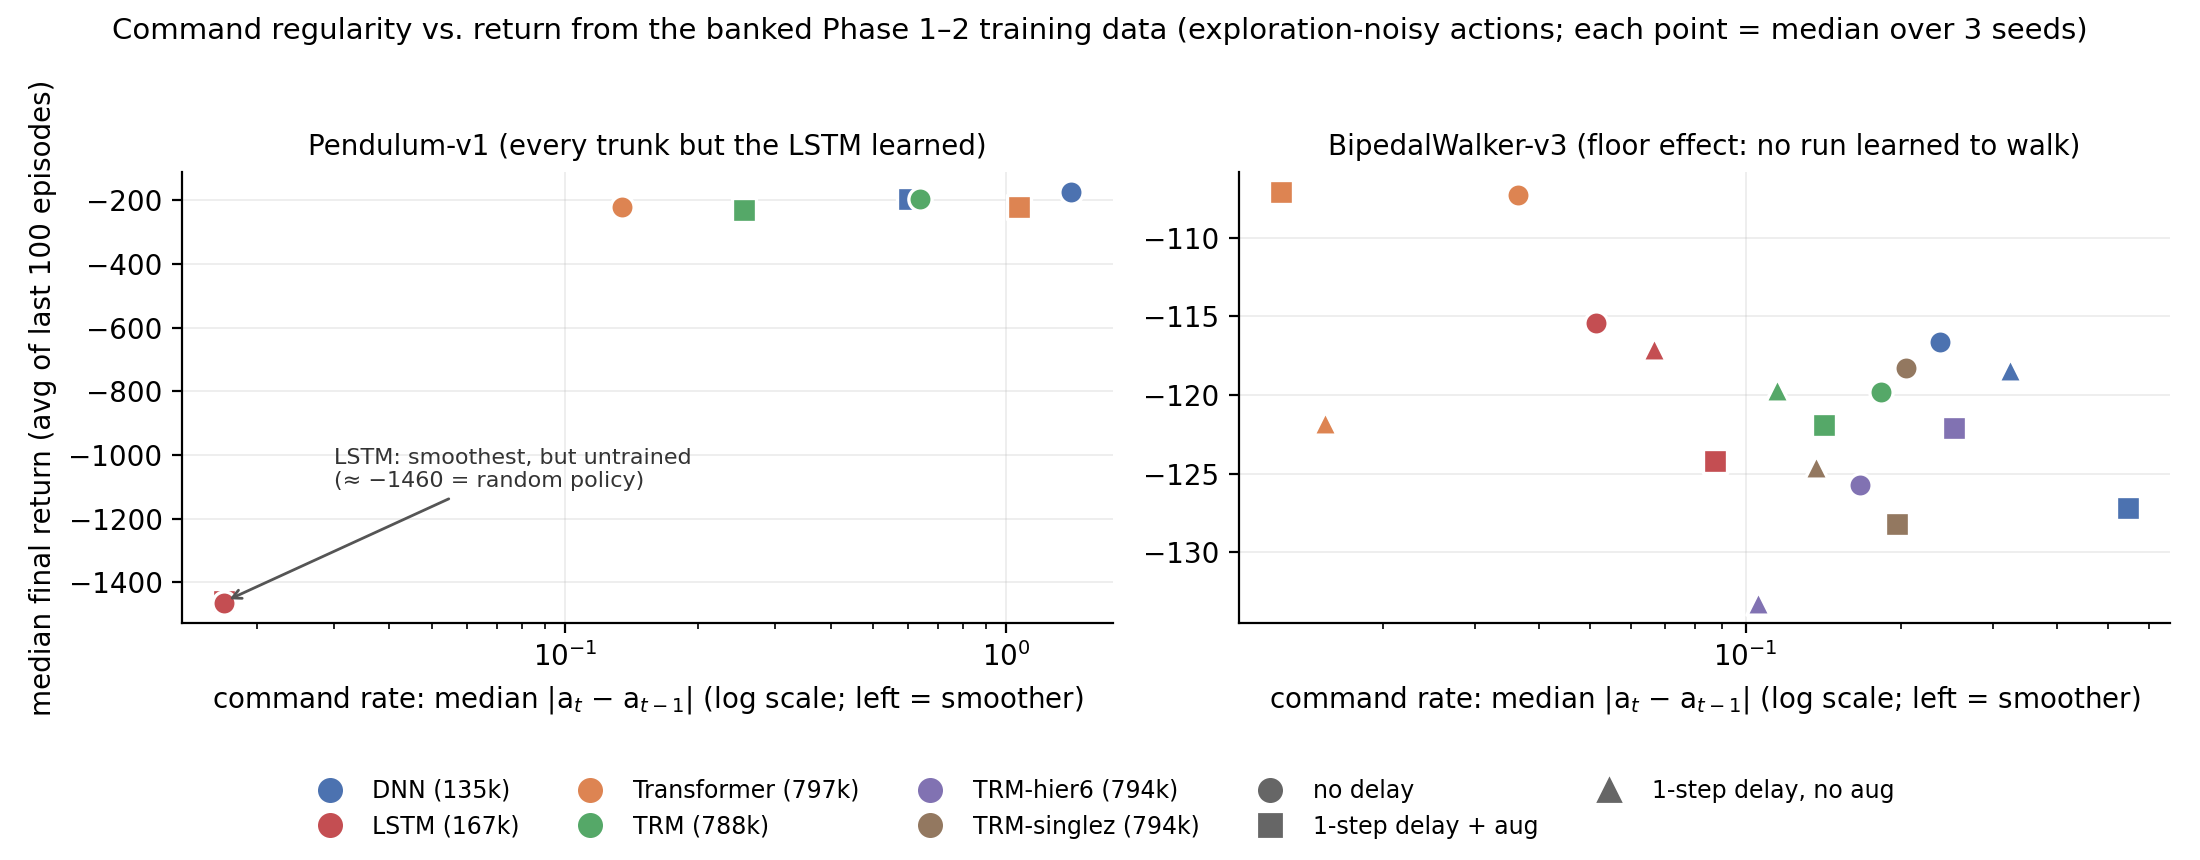
\includegraphics[width=\figw]{figures/fig11_command_rate_vs_return.png}
\caption{Command rate vs return per (trunk, condition) cell, from the banked training data. Pendulum is the only panel containing learned policies, and there is no clean smoothness ordering in it.}
\label{fig:cq}
\end{figure}

\subsection{The stage plan}
\begin{figure}[H]\centering
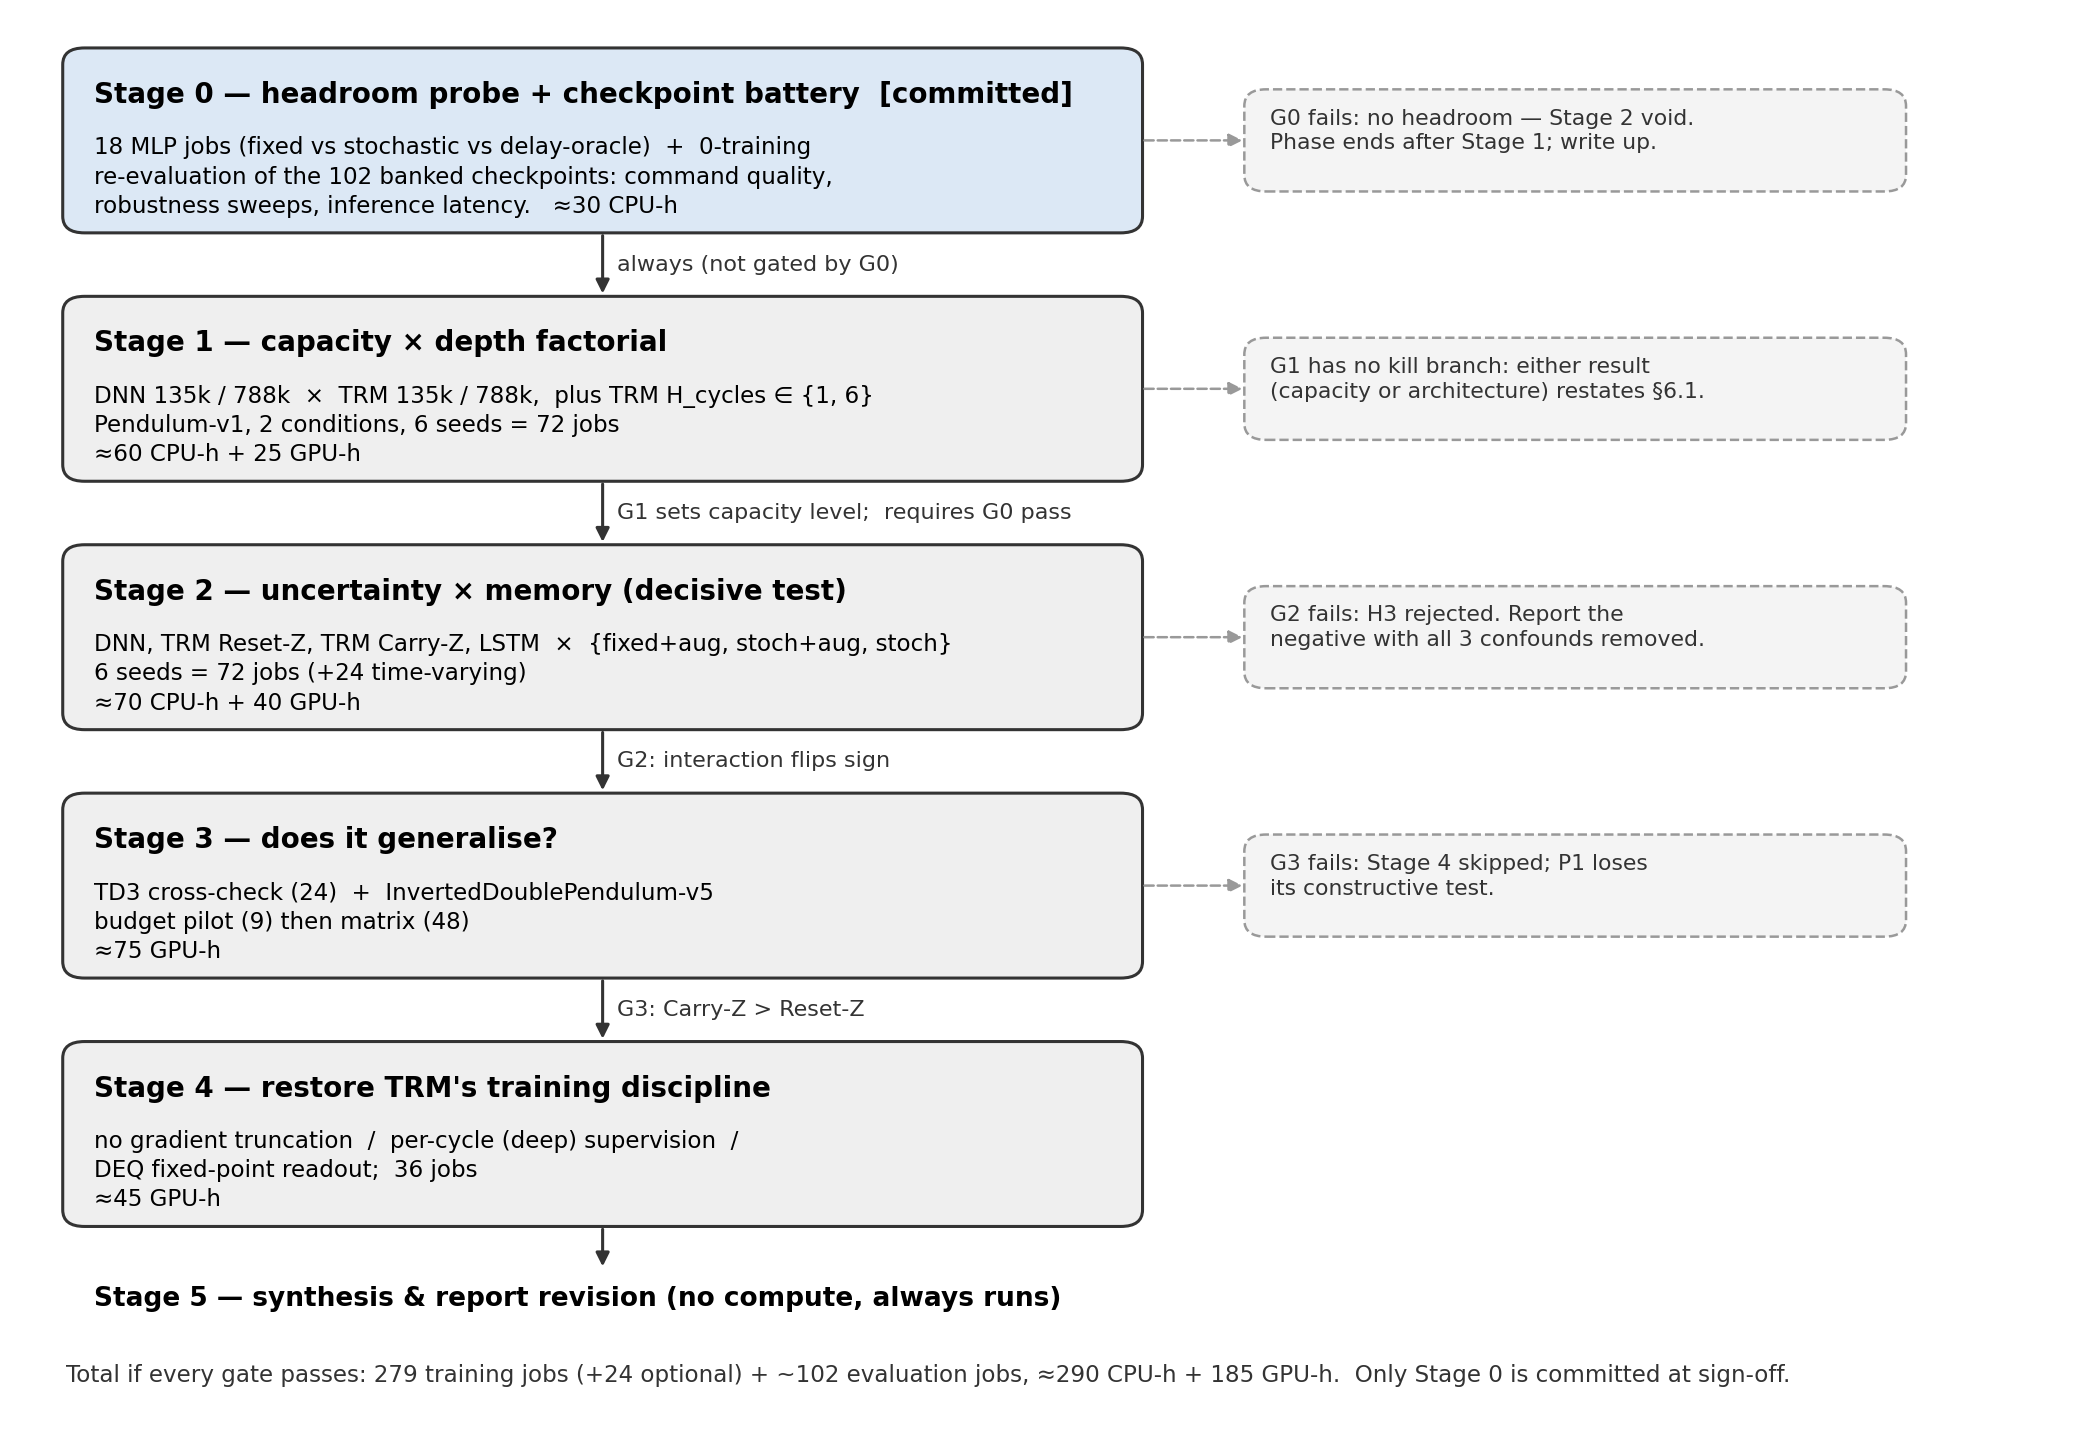
\includegraphics[width=0.92\textwidth]{figures/fig12_phase3_stage_map.png}
\caption{Phase 3 gated stage map (from \texttt{papers/phase3/plan.md} \S4).}
\end{figure}

\begin{table}[H]
\centering\small
\begin{tabularx}{\textwidth}{cYrlY}
\toprule
Stage & Question & Jobs & Cost & Gate \\
\midrule
\textbf{0} & Headroom for inference? What do banked checkpoints tell us (scorecard)? & 18 + 102 eval & ${\approx}30$ CPU-h & \textbf{G0:} oracle-delay MLP beats augmented MLP under stochastic delay \\
\textbf{1} & Capacity or recursion? \{MLP, TRM\} $\times$ \{135k, 788k\} + \texttt{H\_cycles} $\in\{1,6\}$ & 72 & 60 CPU-h + 25 GPU-h & \textbf{G1:} attribution; no kill branch \\
\textbf{2} & Uncertainty $\times$ memory: \{MLP, Reset-Z, Carry-Z, carried LSTM\} $\times$ \{fixed+aug, stoch+aug, stoch\} & 72 (+24) & 70 CPU-h + 40 GPU-h & \textbf{G2:} interaction flips sign, else H3 rejected \\
\textbf{3} & Generalise? TD3 cross-check; InvertedDoublePendulum-v5 after a pilot & 81 & 75 GPU-h & \textbf{G3:} Carry-Z $>$ Reset-Z somewhere \\
\textbf{4} & Restore TRM's training discipline: no truncation, per-cycle supervision, DEQ & 36 & 45 GPU-h & --- \\
\textbf{5} & Synthesis & 0 & --- & always \\
\bottomrule
\end{tabularx}
\end{table}
Only Stage~0 is committed at sign-off. The total if every gate passes is 279 training jobs, ${\approx}290$ CPU-h and 185 GPU-h.

\subsection{Why Phase 3 is important}
\begin{itemize}
  \item \textbf{It is the step that makes the negative result mean something.} Right now ``TRM lost'' cannot be separated from ``a 788k network lost to a 135k one'', or from ``a stateless port was asked to estimate state it was already handed''. Phase 3 either finds a regime where recursion pays, or produces a negative with capacity controlled, the latent carried, real uncertainty present, and environments that get learned. The second outcome is a finding about recursive computation, not about one port.
  \item \textbf{It is cheap to kill.} Each stage has a pre-registered gate, and the first costs about 30 CPU-hours. Phases 1--2 committed 102 jobs up front.
  \item \textbf{It connects the work to engineering practice.} The scorecard decides whether \emph{any} of these trunks could sit in a robot's control loop, whichever way the scientific gates resolve.
  \item \textbf{It follows the literature's strongest lead.} HRM-Agent shows carried-latent recursion can be trained by RL; Stages 2 and 4 are the first tests of whether that carries over to continuous control under delay.
\end{itemize}

\section{Where the project stands}
\begin{table}[H]
\centering\small
\begin{tabularx}{\textwidth}{lYYYY}
\toprule
 & Phase 1 & Phase 2 & Post-hoc & Phase 3 (planned) \\
\midrule
Runs & 48 & 54 & 0 (re-analysis) & Stage 0: 18 + eval \\
Axis & horizon / sparsity & dimensionality / coupling & mechanism & uncertainty $\times$ memory $\times$ capacity; control quality \\
Headline & TRM worse on Pendulum; tie on MountainCar & no significant differences; structure immaterial & floor effects; deficit tracks capacity; latent reset & --- \\
Status & complete & complete & complete & awaiting sign-off \\
\bottomrule
\end{tabularx}
\end{table}

\section{Review of the Phase 3 plan}
\label{sec:review}
\noindent\emph{Checked against \texttt{src/delays.py}, \texttt{src/models/trm\_control.py}, \texttt{src/trainer.py}, \texttt{conf/}, and \texttt{experiments/analysis\_control\_quality.json} on 2026-09-17.}

\subsection{What the plan gets right}
\begin{itemize}
  \item \textbf{The diagnosis is correct and candid.} The three confounds are real, the plan restates them as design faults rather than caveats, and H3 is written so it can clearly fail.
  \item \textbf{\texttt{trm\_h1} is the best single control in the project}: it turns recursion off with parameters, optimiser and input identical. The full 2$\times$2 capacity design is the right fix for C-1.
  \item \textbf{Gating is disciplined.} Kill criteria come before compute, only Stage~0 is committed, and ``success is not a positive result'' is stated up front.
  \item \textbf{Lessons were learned:} a budget pilot before any new environment, 6 seeds minimum, IQM with bootstrap CIs, and the matched-wall-clock reading.
  \item \textbf{The Carry-Z risk is taken seriously}, including the replay-buffer inconsistency and stored-state/burn-in options.
  \item \textbf{Re-using checkpoints} for the scorecard is excellent value for compute.
\end{itemize}

\subsection{Issues}

\subsubsection*{Critical --- these would invalidate the decisive test}

\textbf{1. ``Stochastic delay + augmentation'' contains no inferable hidden state in this codebase.} In \texttt{DelayedEnv.step} the delay $d$ is drawn \textbf{independently each step}, and the applied action is \texttt{buf[-(d+1)]}. It is always either the new action or one of the last \texttt{max\_delay} committed actions, and \textbf{all of those are already in the augmented observation}. Driving the real wrapper for 19{,}600 post-warm-up steps, the applied action fell outside (augmented pending queue $\cup$ current action) \textbf{0 times}. Because future delays are independent of past ones, knowing past realised delays tells the agent nothing about the next one. The uncertainty under C3 is \textbf{irreducible noise, not hidden state}: an MLP sees everything a perfect memory would. The \texttt{augmentation.md} ``approximation'' caveat is about the \emph{meaning} of the queue slots, not Markov sufficiency.
\begin{itemize}
  \item \textbf{H3.2 predicts \emph{no} interaction at C3 even if H3 is true}, so G2 would fail and the plan would ``reject H3'' for a reason unrelated to H3.
  \item \textbf{The Stage~0 oracle arm is uninformative either way.} If A3 exposes the delay of the transition just completed, it adds nothing useful for the next decision and G0 fails spuriously. If it exposes the \emph{upcoming} delay, it provides information no architecture could ever infer, so passing G0 does not show an \emph{inferring} trunk has headroom.
\end{itemize}

\textbf{2. Delay size is confounded with delay uncertainty.} C1 is $d=1$ with one queue slot; C3 has mean delay 2, maximum 4, and four slots. An interaction could come from longer delay or wider input rather than uncertainty. A \textbf{fixed $d=4$ + augmentation} arm (same input width) or fixed $d=2$ (same mean) is the matching control.

\textbf{3. The primary contrast does not separate recursion from memory.} $\Delta = (\text{Carry-Z}-\text{MLP})_{C3} - (\text{Carry-Z}-\text{MLP})_{C1}$ would be positive for \emph{any} trunk that carries state, including a carried LSTM. The pre-registered primary should be \textbf{(Carry-Z $-$ carried LSTM)} and/or \textbf{(Carry-Z $-$ Reset-Z)} interactions, with the MLP contrast as secondary.

\subsubsection*{Major}

\textbf{4. The gate thresholds are looser than the project's own standard.} ``$\ge$5 of 6 seeds'' is one-sided $p=0.109$; Phases 1--2 required $p\le0.031$. Seed pairing across conditions is only meaningful if seeds share initialisation; state that. MLP-only arms take ${\sim}12$ CPU-minutes, so \textbf{Stage~0 and the MLP arms can afford 10+ seeds} (9/10 gives $p=0.011$). Pre-register a bootstrap CI on IQMs for the difference-of-differences.

\textbf{5. The delay-mismatch probe cannot run as specified.} The augmented input width equals \texttt{max\_delay}. A policy trained at fixed $d=1$ expects one queue slot. Testing at $d=0$ turns augmentation off (width 3), and $d\ge2$ needs more slots, so every off-nominal point is a \textbf{shape mismatch}. Pre-register a choice, for example a 1-slot wrapper applying the true delay (feeding the policy wrong queue information, which is a legitimate but specific test).

\textbf{6. Battery scope is inflated.} Of 102 checkpoints, only the Pendulum ones (24, minus untrained LSTMs) are learned policies. Scorecards on floor-effect BipedalWalker/MountainCar policies can't be interpreted. Narrow to Pendulum and pack the evaluation into a handful of jobs.

\textbf{7. The smoothness signal is weaker than presented.} Most pooled pairs (9 of 15 for TRM, Transformer and LSTM) come from BipedalWalker, where nothing learned. On Pendulum with fixed delay + augmentation, \textbf{the Transformer is \emph{rougher} than the MLP} (median $|\Delta a|$ 1.07 vs 0.60), which contradicts ``every non-MLP trunk is markedly smoother''. Figure~\ref{fig:cq} shows no clean ordering on the one valid environment.

\textbf{8. The carried-LSTM baseline has no engineering or tuning budget.} It needs the same off-policy machinery as Carry-Z plus the tuning Ni et al.\ (2022) show is decisive. E-2 covers TRM only. Without this, the ``honest memory baseline'' repeats Phase~1's untuned LSTM.

\textbf{9. The Carry-Z spec is incomplete for actor--critic.} The critic also has a TRM trunk, and target networks need a carry for $s'$. The stored-state option must say which carries are stored (actor, critic, targets) and how the target's carry for $s'$ is obtained.

\subsubsection*{Minor}
\begin{enumerate}[start=10]
  \item \texttt{delay=stochastic min=0 max=4} is \textbf{not} U\{0..4\}: it rounds a continuous uniform, giving $P(d)=0.125,0.25,0.25,0.25,0.125$ (verified by sampling).
  \item \texttt{delay=time\_varying} switches on the \textbf{global training step} (0$\to$1 at 10k, $\to$3 at 20k, $\to$0 at 30k). Pendulum runs 40k steps, so avg-100 return mixes $d=3$ and $d=0$. It is a training-time shift, not within-episode non-stationarity. The C5 rationale also misreads Derman et al.\ (2021): their sub-optimality result concerns stationary policies over the \emph{original} state under \emph{constant} delay; augmented-state policies are optimal there, just exponentially costly. (Report \S3.3/\S9 carry the same reading.)
  \item \texttt{trm\_small} (\texttt{hidden\_size=44}) changes shape as well as size: SwiGLU inner width rounds up to a multiple of 256, giving 256 on a 44-D latent (${\approx}5.8\times$) against 512 on 128-D ($4\times$). Note this, or add a second small variant.
  \item Stage~1 re-runs existing DNN/TRM seeds 1--3. That is fine because the code has changed, but say it \textbf{doubles as a reproduction check}, and don't compare GPU TRM wall-clock with Phase~1's CPU wall-clock.
  \item H3.5 (``recursion degrades more gracefully'') has no proposed mechanism for a Reset-Z trunk. Label it exploratory.
\end{enumerate}

\subsection{Is the budget sensible?}
Yes, broadly. Compute is conditional and front-loaded with cheap stages, and the GPU estimates match Phase~2's measured TRM wall-clock. The main schedule risk is engineering, not compute: E-2 (Carry-Z) plus the missing LSTM equivalent gate Stage~2 by roughly a week.

\subsection{Recommended amendments before sign-off}
\label{sec:amend}
\begin{enumerate}
  \item \textbf{Redesign the uncertainty axis so the hidden quantity can be inferred from history.} The cleanest option is a \textbf{per-episode latent delay}: draw $d\sim$U\{0..4\} once at reset, hold it for the episode, and augment over 4 slots. A memoryless trunk cannot know $d$; a carried trunk can identify it within a few transitions (system identification). The oracle arm (expose $d$) then measures exactly the headroom inference could recover. A \textbf{regime-switching (Markov-chain) delay} with long dwell times is a good second condition and a sound replacement for C5. Keep i.i.d.\ stochastic delay only as a \emph{negative control}, where H3 itself predicts no interaction.
  \item \textbf{Add a fixed $d=4$ + augmentation arm} to Stages 0 and 2.
  \item \textbf{Make the primary contrast (Carry-Z $-$ carried LSTM)}, with (Carry-Z $-$ Reset-Z) co-primary and (Carry-Z $-$ MLP) secondary.
  \item \textbf{Tighten the gates:} 10 seeds for MLP-only arms; $p\le0.05$ or bootstrap CIs excluding zero; one pre-registered statistic per gate.
  \item \textbf{Fix the battery:} pre-register how off-nominal delays are presented to fixed-width policies; restrict the scorecard to learned (Pendulum) policies.
  \item \textbf{Add E-items} for carried-LSTM off-policy machinery and tuning; spell out Carry-Z carries for critic and target networks.
  \item \textbf{Correct the Derman et al.\ reading} and the U\{0..4\} description in the plan and report.
\end{enumerate}

\begin{keybox}
\textbf{Bottom line.} The plan's epistemics and structure are the strongest in the project. Stage~0.2 (the checkpoint battery) can be approved now once item~5 is fixed. Stage~0.1 and Stage~2 should \textbf{not} be submitted as written: under this wrapper their ``uncertain'' condition is informationally equivalent to the augmented observation, so the decisive test would come back null regardless of whether H3 is true. With the per-episode latent-delay redesign, the same budget buys a test that can actually tell H3 apart from H\_cap and H\_null.
\end{keybox}

\section*{References}
\small
\begin{itemize}[leftmargin=*,label={}]
  \item Agarwal et al.\ (2021). \emph{Deep RL at the Edge of the Statistical Precipice.} NeurIPS.
  \item ARC Prize (2025). \emph{The Hidden Drivers of HRM's Performance on ARC-AGI.}
  \item Bai, Kolter \& Koltun (2019). \emph{Deep Equilibrium Models.} NeurIPS.
  \item Dang \& Rawlinson (2025). \emph{HRM-Agent.} arXiv:2510.22832.
  \item Derman, Dalal \& Mannor (2021). \emph{Acting in Delayed Environments with Non-Stationary Markov Policies.} ICLR.
  \item Jolicoeur-Martineau (2025). \emph{Less is More: Recursive Reasoning with Tiny Networks.} arXiv:2510.04871.
  \item Katsikopoulos \& Engelbrecht (2003). Markov decision processes with delays. \emph{IEEE TAC} 48(4).
  \item Klein et al.\ (2024). \emph{Plasticity Loss in Deep RL: A Survey.} arXiv:2411.04832.
  \item Matheron, Perrin \& Sigaud (2019). \emph{The problem with DDPG.} arXiv:1911.11679.
  \item Ni, Eysenbach \& Salakhutdinov (2022). \emph{Recurrent Model-Free RL Can Be a Strong Baseline for Many POMDPs.} ICML.
  \item Ota, Jha \& Kanezaki (2021). \emph{Training Larger Networks for Deep RL.} arXiv:2102.07920.
  \item Roye-Azar et al.\ (2026). \emph{Tiny Recursive Models on ARC-AGI-1.} arXiv:2512.11847.
\end{itemize}

\end{document}
